\documentclass[border=2pt]{standalone}
\usepackage{tikz}
\usetikzlibrary{positioning}

\begin{document}
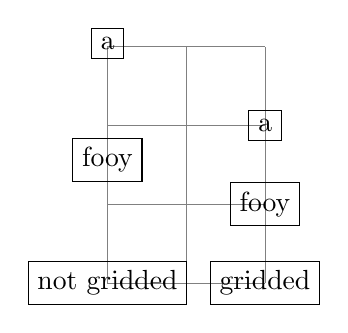
\begin{tikzpicture}[every node/.style={draw,rectangle}]
  \draw[help lines] (0,0) grid (2,3);

  % Border-to-border placement is the default.
  \node (a1) at (0,0) {not gridded};
  \node (b1) [above=1cm of a1] {fooy};
  \node (c1) [above=1cm of b1] {a};

  % With on grid, every placement uses both node centres.
  \node (a2) at (2,0) {gridded};
  \node (b2) [on grid,above=1cm of a2] {fooy};
  \node (c2) [on grid,above=1cm of b2] {a};
\end{tikzpicture}
\end{document}
